% !TEX TS-program = pdflatex
% !TEX encoding = UTF-8 Unicode

% This is a simple template for a LaTeX document using the "article" class.
% See "book", "report", "letter" for other types of document.

\documentclass[11pt]{article} % use larger type; default would be 10pt

%\usepackage[utf8]{inputenc} % set input encoding (not needed with XeLaTeX)


%%% Examples of Article customizations
% These packages are optional, depending whether you want the features they provide.
% See the LaTeX Companion or other references for full information.

%%% PAGE DIMENSIONS
\usepackage{geometry} % to change the page dimensions
\geometry{a4paper} % or letterpaper (US) ocher a5paper or....
\geometry{margin=1in} % for example, change the margins to 2 inches all round
% \geometry{landscape} % set up the page for landscape
%   read geometry.pdf for detailed page layout information

\usepackage{graphicx} 
% \usepackage[parfill]{parskip} % Activate to begin paragraphs with an empty line rather than an indent

%%% PACKAGES
%\usepackage{booktabs} % for much better looking tables
\usepackage{array} % for better arrays (eg matrices) in maths
%\usepackage{paralist} % very flexible & customisable lists (eg. enumerate/itemize, etc.)
\usepackage{verbatim} % adds environment for commenting out blocks of text & for better verbatim
%\usepackage{subfig} % make it possible to include more than one captioned figure/table in a single float
% These packages are all incorporated in the memoir class to one degree or another...

%%% HEADERS & FOOTERS
\usepackage{fancyhdr} % This should be set AFTER setting up the page geometry
\pagestyle{fancy} % options: empty , plain , fancy
\renewcommand{\headrulewidth}{0pt} % customise the layout...
\lhead{}\chead{}\rhead{}
\lfoot{}\cfoot{\thepage}\rfoot{}

%%% SECTION TITLE APPEARANCE
%\usepackage{sectsty}
%\allsectionsfont{\sffamily\mdseries\upshape} % (See the fntguide.pdf for font help)
% (This matches ConTeXt defaults)

%%% ToC (table of contents) APPEARANCE
%\usepackage[nottoc,notlof,notlot]{tocbibind} % Put the bibliography in the ToC
%\usepackage[titles,subfigure]{tocloft} % Alter the style of the Table of Contents
%\renewcommand{\cftsecfont}{\rmfamily\mdseries\upshape}
%\renewcommand{\cftsecpagefont}{\rmfamily\mdseries\upshape} % No bold!

%\usepackage[T1]{fontenc}
\usepackage[latin9]{inputenc}
%\usepackage[active]{srcltx}
\usepackage{setspace}
\usepackage{lscape}
\doublespacing
\usepackage[english]{babel}

\begin{document}

\title{SI:  Approaches for Large Scale Metagenome Assembly}
\author{ACH, JMT, CTB}
\maketitle

\subsubsection{Summary of approaches used on mock community dataset}

The HMP mock community dataset and its available draft reference genomes were used to evaluate our approaches towards data reduction and partitioning for \emph{de novo} metagenomic assembly.   Reads of the mock community dataset were initially digitally normalized to a coverage threshold of 20 (as previously described in Brown et al), reducing the total number of reads from 14 to 11 million.  Additionally, to remove possible sequencing artifacts associated with high coverage sequences (previously described in Howe et al), highly-abundant sequences (20-mers present at coverage greater than 50-fold) were filtered and the dataset was further normalized to a coverage of 10, resulting in a total of 9 million reads (Figure ~\ref{kmercoverage}).  Finally, the remaining reads were divided into disconnected sets of reads resulting in a total of 85,818 partitions containing greater than five reads (summarized in Table~\ref{datareduction}).

\section{Methods}

\subsection{Datasets}
In this study, we examined two large soil metagenomes generated from soils collected from Iowa corn and native prairie soils.  Sequencing was performed at the DOE Joint Genome Institute (Walnut Creek, CA).   Reads were quality trimmed at where Phred scores indicated a score of '2'.  The total quality-trimmed reads in the Iowa corn and prairie datasets were 1.8 million and 3.3 million, respectively.  We also include a human gut mock community dataset (combined from SRA SRX055381 and SRX055380).  For this mock community dataset, DNA from bacterial isolates originally recovered from within or on the human body was mixed together at staggered concentrations (over 5 orders of magnitude based on genomic DNA concentrations) and sequenced.  The mock community dataset originally contained 14.5 million reads.  

To evaluate our approaches, we added simulated reads from either a single E. Coli (str. K-12 substr DH10B) or five E. coli strains (K-12 substr DH10B, E24377, O147:H7 str. EC4115, UMN026, SE15) into select metagenomes.  We computationally generated 100 bp reads from each reference genome to a coverage of 10x and with a 2\% error rate and subsequently randomly shuffled these reads with select datasets.


\subsubsection{Digital normalization}
Digital normalization was previously describe in X.  For the mock community dataset, digital normalization was performed with the following parameters:  K=20, coverage=20, and Bloom filter size = 1 GB x 4.  For Iowa corn metagenome, digital normalization parameters were as follows:  K=20, coverage=20, and Bloom filter size = 48 GB x 4.  Similar parameters were used for the Iowa prairie metagenome, with the exception that the Bloom filter size was 60 GB x 4.

\subsubsection{Removal of high abundance sequences}
To eliminate known sequencing artifacts in Illumina metagenomes (previously described in XXX), high abundance sequences (coverage greater than 50) were removed using the count-min-sketch datastructure used for digital normalization.  For the relatively high coverage mock community dataset, filtered reads were subsequently normalized to a coverage of 10 (K=20, bloom filter size = 1 GB x 4).  

\subsection{Identication of \emph{gyrB}, \emph{recA}, and \emph{rplB}}
Well-curated sequences from the Ribosomal Database Project's (RDP) Functional Gene Repository were used to build HMM profiles for \emph{gyrB}, \emph{recA}, and \emph{rplB}.  These models are available upon request from RDP.  The \emph{gyrB}, \emph{recA}, and \emph{rplB} HMM models contained 809, 353, and 277 amino acids, respectively.  Assembled contigs were translated in all six reading frames and searched against the HMM profiles using HMMER3 (v3.0).  Results were filtered with an E-value threshold of 1e-5.  The abundance of assembled contigs were previously calculated as described above and used to estimate total number of \emph{gyrB}, \emph{recA}, and \emph{rplB} genes within soil metagenomes.  We also evaluated our ability to identify these genes against the HMP mock reference dataset and found that in some cases, the genes were not identified for some isolates or multiple reading frames within a reference genome were found to contain the gene of interest.  We thus corrected calculated abundances of these genes based on our ability to identify the 22 HMP isolates using the described methods.  

\subsection{Figures and Tables}


\begin{landscape}
\begin{table}[h!]
\center{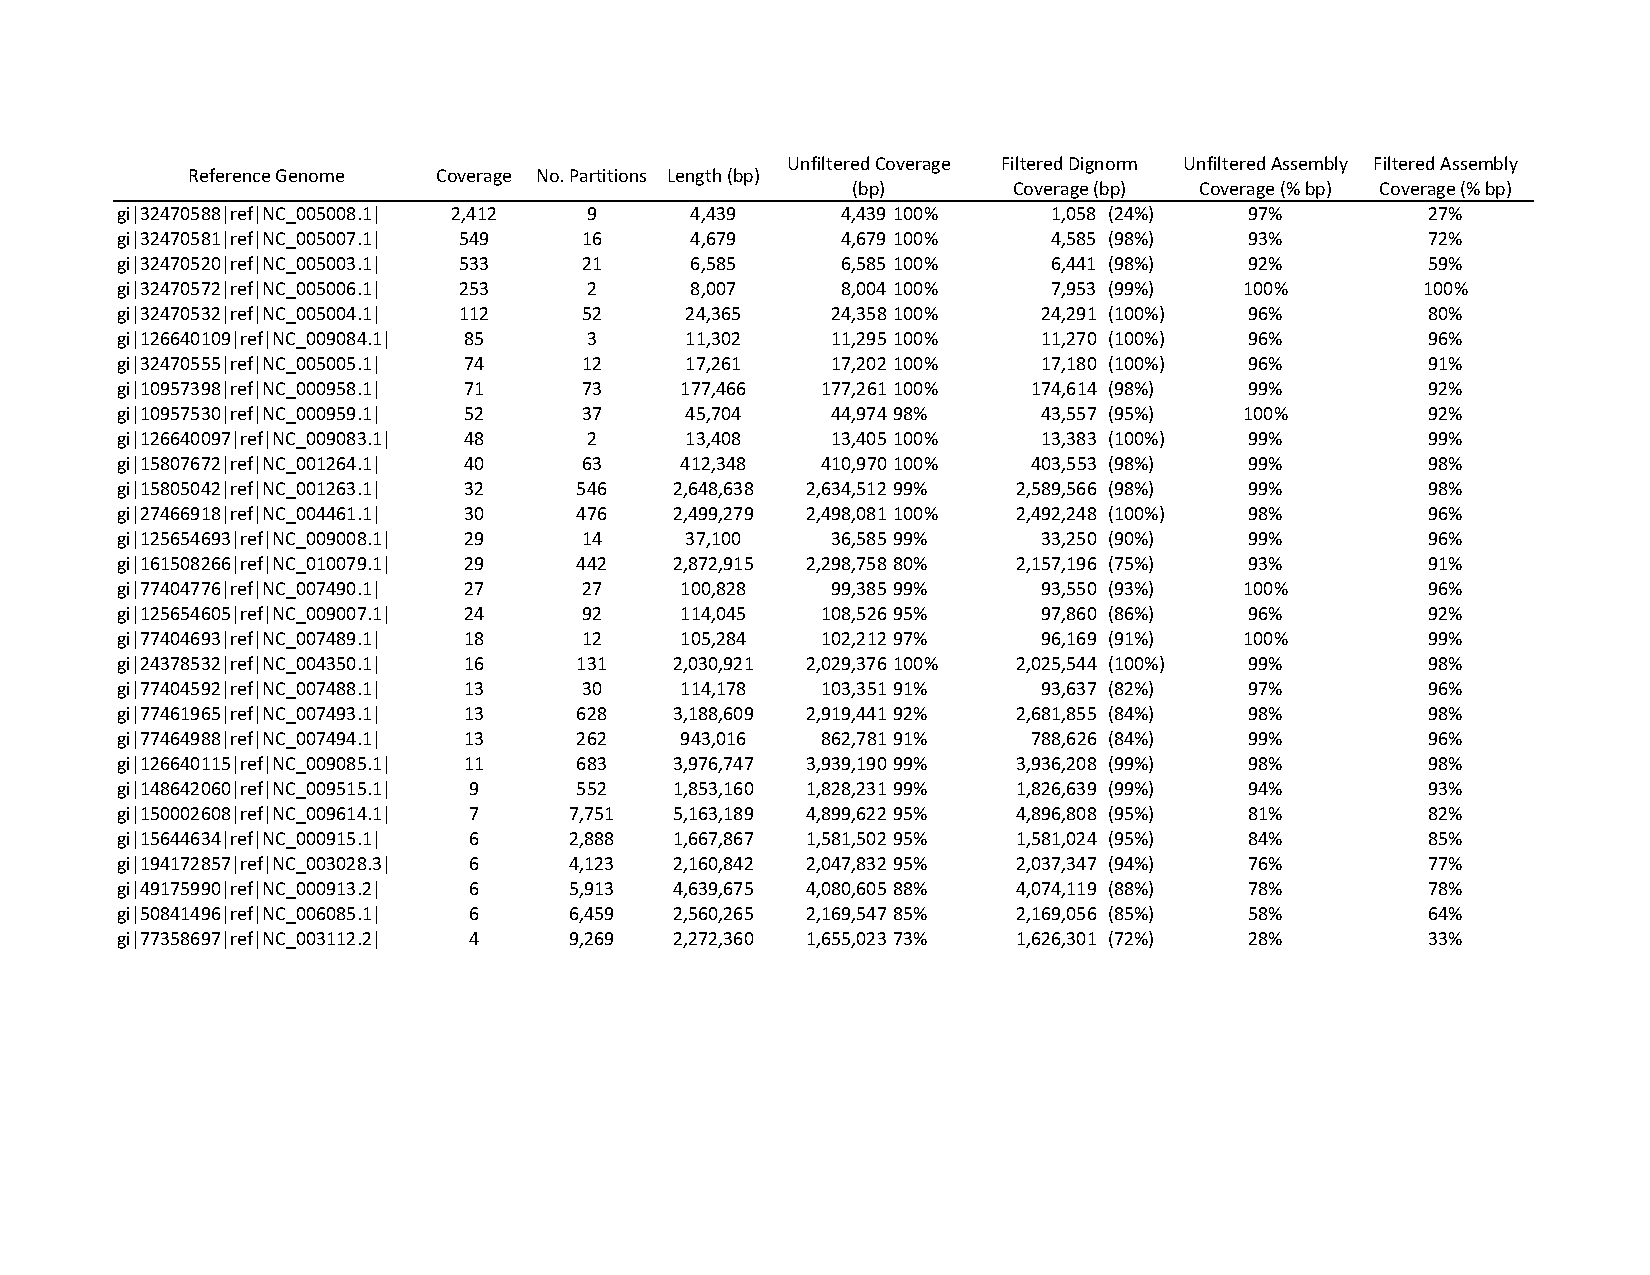
\includegraphics[scale=1.0]{./figures/reference-genomes.pdf}}
\caption{Candidate for Suppl.:  HMP mock dataset reference genomes estimated sequencing depth (median bp coverage of reads), number of partitions, total length (bp), coverage of reference genomes by unfiltered reads, coverage of reference genomes by filtered reads, coverage of reference genomes by unfiltered assembled contigs, and coverage of reference genomes by filtered assembled contigs.}
\label{referencestats}
\end{table}
\end{landscape}




\end{document}

